\section{Cloud Architektur}
In diesem Kapitel wird auf die verwendete Architektur in \ac{AWS} eingegangen. Die nachfolgende Abbildung gibt einen Überblick wie die einzelnen Komponenten miteinander kommunizieren und voneinander abhängen. Die Services die eingesetzt werden sind eine Code Pipeline, \ac{ECS} und ein Code-\gls{Repository} in welchem der Anwendungscode abgelegt ist.

\begin{figure}[H]
    \centering
    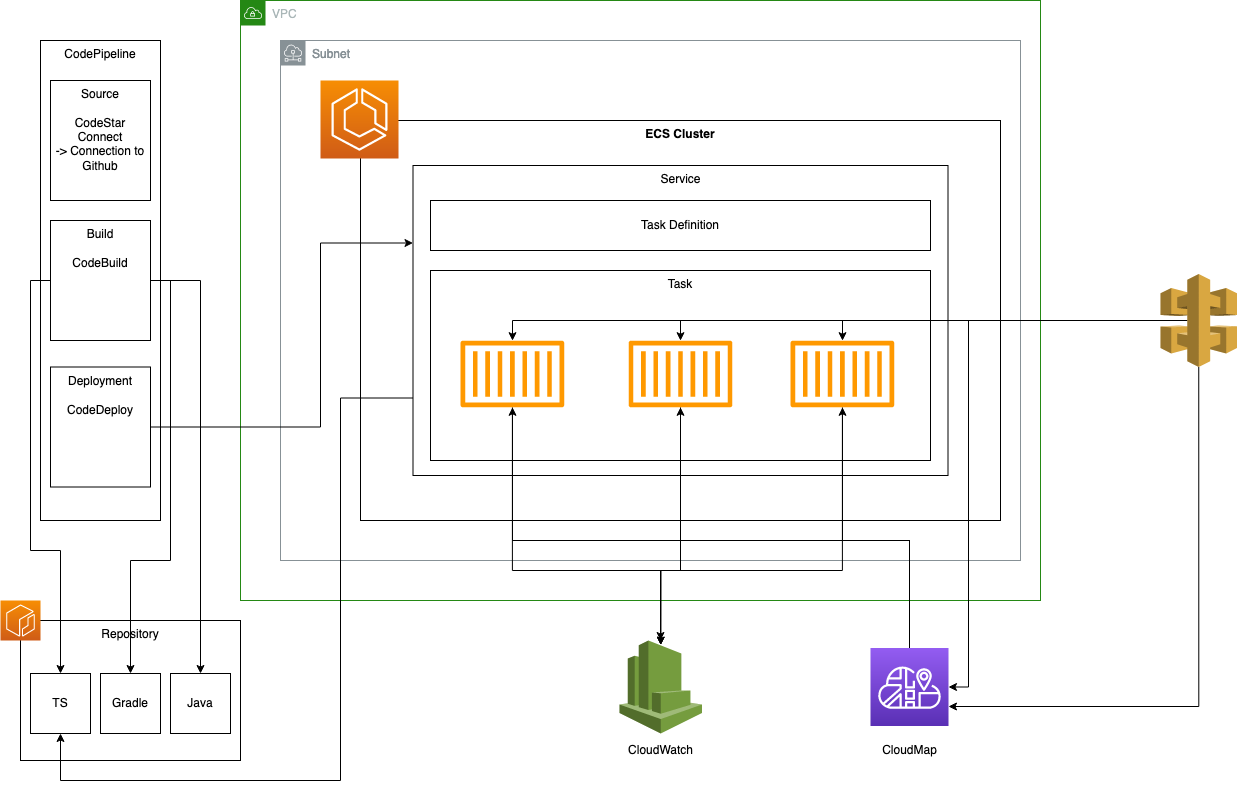
\includegraphics[width=\textwidth]{aws_architecture.png}
    \caption{Architekturentwurf für die AWS-Services}
    \label{fig:CloudArchitektur}
\end{figure}

Innerhalb einer \ac{VPC} wird ein Subnetz bereitgestellt, in welchem wiederum der \ac{ECS}-Service sein eigenes isoliertes Netzwerk zum Starten des \ac{ECS}-Clusters hat. Um die Bereitstellung und Konfiguration des \ac{ECS}-Clusters zu vereinfachen wird Fargate eingesetzt. Damit wird sichergestellt, dass der \ac{ECS}-Service weitere Instanzen desselben \ac{ECS}-Clusters starten kann, wenn zum Beispiel Aufgaben fehlschlagen. In diesem \ac{ECS}-Cluster läuft dann eine zuvor definierte Zahl von Instanzen der Anwendung.

Neben dem Containerservice wird außerdem eine Code Pipeline zum Ausspielen der Anwendung in den Containern eingesetzt. Hierzu wird der Anwendungscode von \textit{CodeStar} aus dem Code-\gls{Repository} geladen, \textit{CodeBuild} erzeugt dann eine ausführbare Anwendung, die von \textit{CodeDeploy} in die Container geladen wird. Als \gls{Repository} wird in diesem Fall \gls{GitHub} eingesetzt.